\chapter{CMDP Formulation}

This chapter formalizes the Behavioral Engine for Demand (BED) as a Constrained
Markov Decision Process (CMDP). While the behavioral model in Chapter 4
describes how incentives influence user state transitions, the CMDP determines
\emph{when} incentives should be delivered to maximize long-term behavioral
impact under operational constraints. The CMDP framework ensures that BED
allocates incentives efficiently, fairly, and in a manner consistent with
organizational policy.
\begin{table}[h!]
\centering
\caption{CMDP state variables used in the BED formulation.}
\begin{tabular}{ll}
\toprule
\textbf{State Variable} & \textbf{Description} \\
\midrule
$h_t$ & Habit strength at time $t$ \\
$r_t$ & Recency (time since last event) \\
$i_t$ & Time since last incentive \\
$b_t$ & Remaining budget \\
$f_t$ & Fairness constraint state \\
\bottomrule
\end{tabular}
\label{tab:cmdp_state_variables}
\end{table}

\section{Overview}

A CMDP extends the classical Markov Decision Process by incorporating resource
constraints. In BED, the primary constraints are:

\begin{itemize}
    \item \textbf{Budget constraint}: incentives must not exceed a fixed budget.
    \item \textbf{Fairness constraint}: exposure to incentives must be balanced
    across user segments.
    \item \textbf{Eligibility constraint}: incentives may only be delivered when
    certain behavioral conditions are met.
\end{itemize}

These constraints reflect real-world operational requirements and ensure that
BED remains practical and deployable.

\section{CMDP Definition}

The CMDP is defined by the tuple:


\[
\mathcal{M} = (S, A, P, r, c, \gamma, B),
\]


where:

\begin{itemize}
    \item $S$ is the state space (behavioral state variables),
    \item $A$ is the action space (incentive or no incentive),
    \item $P(s'|s,a)$ is the transition probability,
    \item $r(s,a)$ is the reward function,
    \item $c(s,a)$ is the cost of taking action $a$ in state $s$,
    \item $\gamma$ is the discount factor,
    \item $B$ is the total allowable cost (budget).
\end{itemize}

\subsection{State Space}
\begin{figure}[h!]
\centering
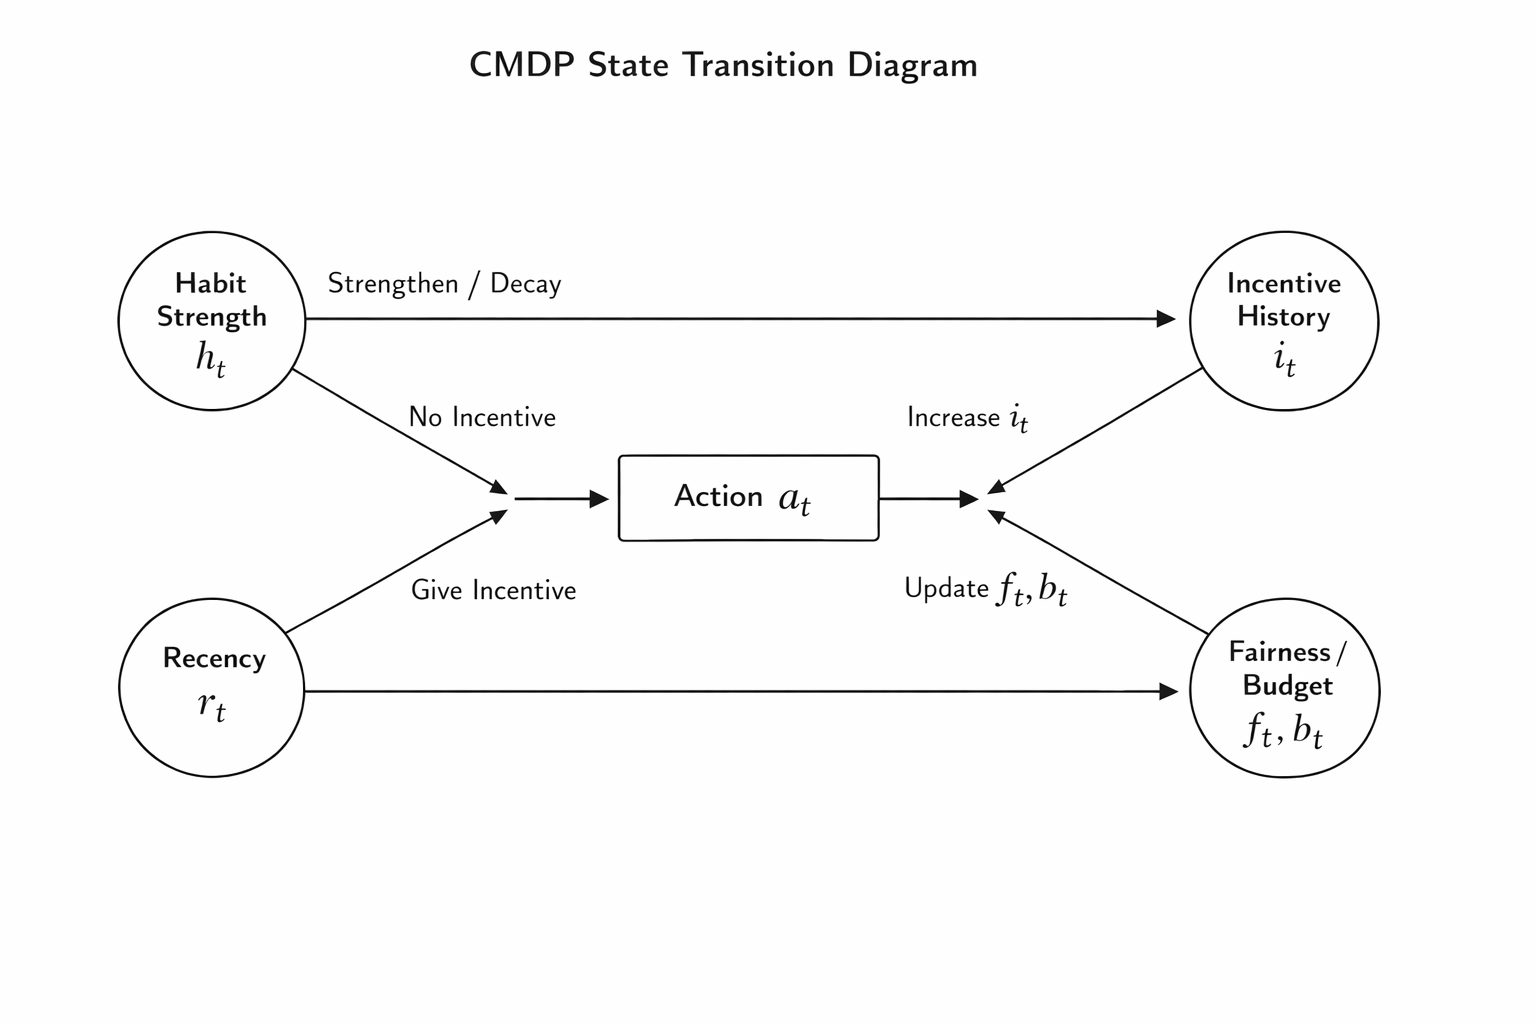
\includegraphics[width=0.75\textwidth]{figures/cmdp_state_transition.png}
\caption{CMDP state transition structure illustrating how habit strength, recency, and incentive history evolve over time under different actions.}
\label{fig:cmdp_transition}
\end{figure}

The state space is defined as:


\[
s_t = (r_t, h_t, \rho_t, \Delta_t, I_{t-1}),
\]


as introduced in Chapter 4.

\subsection{Action Space}

The action space is binary:


\[
A = \{0, 1\},
\]


where:
\begin{itemize}
    \item $a = 0$ means no incentive is delivered,
    \item $a = 1$ means an incentive is delivered.
\end{itemize}

\subsection{Transition Dynamics}

Transitions follow the behavioral update rules in Chapter 4:


\[
P(s_{t+1} | s_t, a_t)
\]


is determined by:
\begin{itemize}
    \item event probability from the hazard model,
    \item deterministic updates to recency, habit, and incentive decay,
    \item stochasticity in user responsiveness.
\end{itemize}

\section{Reward Function}

The reward function captures the objective of BED: increasing the probability of
engagement and strengthening long-term habit formation. A simple formulation is:


\[
r(s,a) = \mathbb{1}\{\text{event occurs}\},
\]


though more complex reward structures may incorporate:

\begin{itemize}
    \item habit growth,
    \item long-term retention,
    \item segment-specific objectives.
\end{itemize}

\section{Cost Function and Budget Constraint}

The cost function is:


\[
c(s,a) =
\begin{cases}
C & \text{if } a = 1, \\
0 & \text{if } a = 0,
\end{cases}
\]


where $C$ is the cost of delivering an incentive.

The budget constraint requires:


\[
\mathbb{E}_{\pi} \left[ \sum_{t=0}^{\infty} \gamma^t c(s_t, a_t) \right] \le B.
\]



This ensures that BED does not exceed the incentive budget.

\section{Fairness Constraint}

To ensure equitable treatment across user segments, BED imposes a fairness
constraint:


\[
\left| \mathbb{E}_{\pi}[a_t \mid g = i] - \mathbb{E}_{\pi}[a_t \mid g = j] \right|
\le \epsilon,
\]


for all segments $i, j$.

This constraint ensures that no segment is disproportionately favored or
disadvantaged.

\section{Objective}

The CMDP objective is:


\[
\max_{\pi} \; \mathbb{E}_{\pi} \left[ \sum_{t=0}^{\infty} \gamma^t r(s_t, a_t) \right]
\]


subject to:


\[
\mathbb{E}_{\pi} \left[ \sum_{t=0}^{\infty} \gamma^t c(s_t, a_t) \right] \le B,
\]


and fairness constraints.

\section{Lagrangian Relaxation}

To solve the CMDP, BED uses a Lagrangian relaxation:


\[
\mathcal{L}(\pi, \lambda) =
\mathbb{E}_{\pi} \left[ \sum_{t=0}^{\infty} \gamma^t
\left( r(s_t, a_t) - \lambda c(s_t, a_t) \right) \right]
+ \lambda B.
\]



The dual problem is:


\[
\min_{\lambda \ge 0} \max_{\pi} \mathcal{L}(\pi, \lambda).
\]



This converts the CMDP into a sequence of unconstrained MDPs parameterized by
$\lambda$.

\section{Constrained Bellman Equation}

The Lagrangian value function satisfies:


\[
V_{\lambda}(s) =
\max_{a \in A}
\left[
r(s,a) - \lambda c(s,a)
+ \gamma \sum_{s'} P(s'|s,a) V_{\lambda}(s')
\right].
\]



The optimal policy is:


\[
\pi_{\lambda}^{*}(s) =
\arg\max_{a \in A}
\left[
r(s,a) - \lambda c(s,a)
+ \gamma \sum_{s'} P(s'|s,a) V_{\lambda}(s')
\right].
\]



\section{Eligibility Constraints}

Incentives may only be delivered when:


\[
a_t = 1 \implies r_t \ge r_{\min},
\]


or when other operational rules are satisfied.

This prevents wasteful or inappropriate incentive delivery.

\section{Policy Structure}

The optimal BED policy has the following properties:

\begin{itemize}
    \item \textbf{Threshold-based}: incentives are delivered when recency,
    habit, or responsiveness cross certain thresholds.
    \item \textbf{Cost-aware}: incentives are withheld when budget is low.
    \item \textbf{Fairness-aware}: exposure is balanced across segments.
    \item \textbf{Timing-optimized}: incentives are delivered at moments of
    maximum behavioral leverage.
\end{itemize}

These properties emerge naturally from the CMDP formulation.

\section{Summary}

This chapter formalized the CMDP that governs incentive allocation in BED v3.
The next chapter describes the simulation environment used to evaluate the
performance of CMDP policies under realistic behavioral dynamics.
